\documentclass[tikz,border=6pt]{standalone}
\usepackage{tikz}

\begin{document}

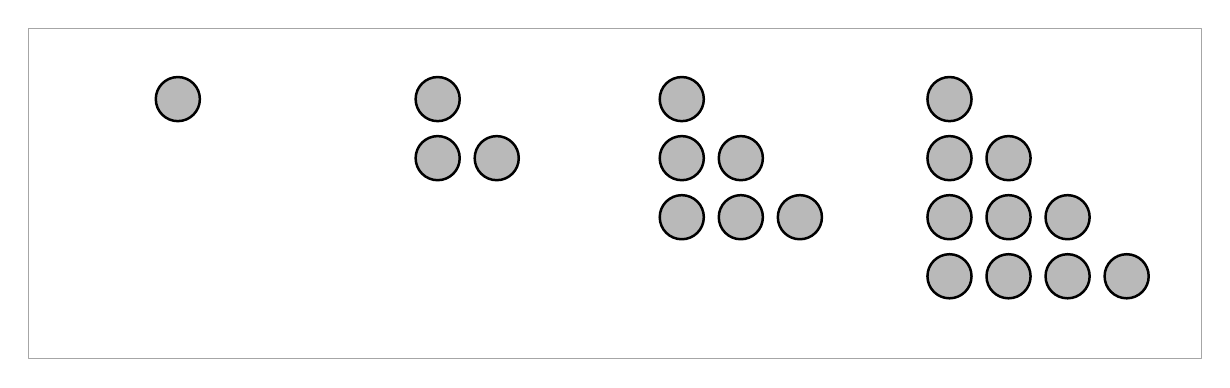
\begin{tikzpicture}[line cap=round,line join=round]
  % --- parameters ---
  \def\s{0.75}   % grid step
  \def\r{0.28}   % circle radius

  % --- outer frame ---
  \draw[gray!70] (-0.7,0.9) rectangle (14.2,-3.3);

  % style for filled dots
  \tikzset{fdot/.style={draw=black,fill=gray!55,line width=.9pt}}

  % ========== (1) : 1 dot ==========
  \begin{scope}[shift={(1.2,0.0)}]
    \filldraw[fdot] (0,0) circle (\r);
  \end{scope}

  % ========== (2) : 3 dots (1+2) ==========
  \begin{scope}[shift={(4.5,0.0)}]
    \foreach \x/\y in {0/0,0/-1,1/-1}
      \filldraw[fdot] (\x*\s,\y*\s) circle (\r);
  \end{scope}

  % ========== (3) : 6 dots (1+2+3) ==========
  \begin{scope}[shift={(7.6,0.0)}]
    \foreach \x/\y in {0/0,0/-1,1/-1,0/-2,1/-2,2/-2}
      \filldraw[fdot] (\x*\s,\y*\s) circle (\r);
  \end{scope}

  % ========== (4) : 10 dots (1+2+3+4) ==========
  \begin{scope}[shift={(11.0,0.0)}]
    \foreach \x/\y in {0/0,
                       0/-1,1/-1,
                       0/-2,1/-2,2/-2,
                       0/-3,1/-3,2/-3,3/-3}
      \filldraw[fdot] (\x*\s,\y*\s) circle (\r);
  \end{scope}
\end{tikzpicture}

\end{document}
